% !TEX root = main.tex
\chapter{Results}
\label{chap:results}

\linespread{1.08}\selectfont
The \CP asymmetries \Sf and \Sfbar are determiend in the \BdToDpi decay on the full \lhcb Run I data set at centre-of-mass energies of \num{7} and \SI{8}{\tera\electronvolt} and measured to be
\begin{equation}
\begin{aligned}
\Sf&=0.058\pm0.020\stat\pm0.011\syst\,,\\
\Sfbar&=0.038\pm0.020\stat\pm0.007\syst\,,
\end{aligned}
\end{equation}
where the statistical and systematic correlations are \SI{60}{\percent} and \SI{-41}{\percent}, respectively.
These values are in agreement with, and more precise than, previous measurements from the \belle and \babar colloborations~\cite{Ronga:2006hv,Aubert:2006tw}.
According to Wilk's theorem~\cite{wilks1938}, they result in a significance of $2.7\sigma$ for \mbox{\CP violation}.
This result, even if it is not yet an evidence for \CP violation, yields a larger significance for \CP violation than the previous measurement from the \belle collaboration~\cite{Ronga:2006hv}.

Furthermore, the \CP asymmetries can be expressed using a parametrisation introduced by the \babar collaboration~\cite{Aubert:2006tw} and adopted by HFLAV~\cite{HFLAV2016} with
\begin{equation}
\begin{aligned}
a=-\frac{2r}{1+r^2}\sin\!\left(2\beta+\gamma\right)\cos\!\left(\delta\right)\,,\\
c=-\frac{2r}{1+r^2}\cos\!\left(2\beta+\gamma\right)\sin\!\left(\delta\right)\,.
\end{aligned}
\end{equation}
In this parametrisation only the parameter $c$ is affected by the so-called tag-side interference, an experimental effect due to the coherent \Bz\Bzb production at \belle and \babar~\cite{Long:2003wq}.
From a comparison with Eqs. \eqref{eq:DefSf} and \eqref{eq:DefSfbar} the transformation rules
\begin{equation}
a=-\frac{1}{2}\left(\Sf+\Sfbar\right)\hspace{0.5cm}\text{and}\hspace{0.5cm}c=\frac{1}{2}\left(\Sf-\Sfbar\right)\\
\end{equation}
follow.
Hence, the \CP asymmetries can be expressed as
\begin{equation}
\begin{aligned}
a&=-0.048\pm0.018\stat\pm0.005\syst\,,\\
c&=0.010\pm0.009\stat\pm0.008\syst\,,\\
\end{aligned}
\end{equation}
where the statistical correlation is zero and the systematic correlation is \SI{-46}{\percent}.

The values for \Sf and \Sfbar are further interpreted in terms of the angles $\beta$ and $\gamma$, as well as the amplitude ratio $r$ and the \emph{strong} phase $\delta$ (see \cref{eq:DefSf} and \eqref{eq:DefSfbar}).
This is done using a frequentistic approach as described in Ref.~\cite{Aaij:2016kjh}, where the PDFs $f_i$ containing the experimental observables $\vec{A}_i$ are combined into one likelihood function
\begin{equation}
\mathcal{L}(\vec{\alpha})=\prod_i f_i\left(\vec{A}_i^{\text{obs}}\big|\vec{\alpha}\right)\,,
\end{equation}
where $\vec{A}_i^{\text{obs}}$ are the experimentally measured parameters and $\vec{\alpha}$ is the set of parameters to be extracted.
For all inputs, Gaussian distributions are assumed according to
\begin{equation}
f_i\left(\vec{A}_i^{\text{obs}}\big|\vec{\alpha}\right)\propto\exp\!\left(-\frac{1}{2}\left(\vec{A}_i(\vec{\alpha})-\vec{A}_i^{\text{obs}}\right)^T V_i^{-1}\left(\vec{A}_i(\vec{\alpha})-\vec{A}_i^{\text{obs}}\right)\right)\,,\label{eq:gaussForPLugin}
\end{equation}
where $V_i$ is the experimentally determined covariance matrix with the statistical and systematic uncertainties and the corresponding correlations.
The best fit point is given as the minimum of a $\chi^2$-function, defined as $\chi^2(\vec{\alpha})=-2\ln\mathcal{L}(\vec{\alpha})$.
The confidence level (CL) for a given parameter value, hereinafter $\gamma_0$, is calculated using a test statistic defined as $\Delta\chi^2=\chi^2(\vec{\alpha}'_{\text{min}}(\gamma_0))-\chi^2(\vec{\alpha}_{\text{min}})$, where $\chi^2(\vec{\alpha}_{\text{min}})$ is the global minimum and $\chi^2(\vec{\alpha}'_{\text{min}}(\gamma_0))$ is the new minumum with the parameter value $\gamma_0$.

The $p$-value or $1-\text{CL}$ is calculated by a procedure using pseudoexperiments:
for each value $\gamma_0$, the test statistic $\Delta\chi^2$ is calculated and a set of pseudoexperiments $\vec{A}_j$ is generated according to \cref{eq:gaussForPLugin}.
In this generation, the parameters $\vec{\alpha}$ are set to the values of the new minimum $\vec{\alpha}'$.
For each pseudoexperiment, a new test statistic is then calculated by replacing $\vec{A}_{\text{obs}}$ with $\vec{A}_j$, which is again minimised with respect to $\vec{\alpha}$; once with the parameter $\gamma$ free, once with $\gamma$ set to $\gamma_0$.
The $1-\text{CL}$ value is defined as the fraction of pseudoexperiments in which $\Delta\chi^2<\Delta\chi^{2'}$.
More details about this method can also be found in Ref.~\cite{Bodhisattva:2009uba}.

By adding external measurements for $r$, confidence intervals for the quantity $\sin\!\left(2\beta+\gamma\right)$ and the \emph{strong} phase $\delta$ can be derived.
The ratio $r$ is determined from the branching fraction of $\Bz\!\to\Dsp\pim$ under the assumption of SU(3) symmetry with the same equations one finds in Refs~\cite{Aubert:2008zi, Das:2010be}
\begin{equation}
r=\tan(\theta_c)\frac{f_\Dp}{f_\Ds}\sqrt{\frac{\mathcal{B}\!\left(\Bz\!\to\Dsp\pim\right)}{\mathcal{B}\!\left(\Bz\!\to\Dm\pip\right)}}
\end{equation}
where $\tan(\theta_c)=\num{0.23101\pm0.00032}$ is the tangent of the Cabibbo angle from Ref.~\cite{CKMfitter2015}.
For the branching fractions \mbox{$\mathcal{B}\!\left(\Bz\!\to\Dsp\pim\right)=\num{2.16\pm0.26 e-5}$} and \mbox{$\mathcal{B}\!\left(\Bz\!\to\Dm\pip\right)=\num{2.52\pm0.13 e-3}$}, the values reported in Ref.~\cite{PDG2018} are used.
The ratio of decay constants $\,\nicefrac{f_\Dp}{f_\Ds}\!=\num{1.173\pm0.003}$ is taken from \mbox{Refs.~\cite{Aoki:2016frl, Bazavov:2014wgs, Carrasco:2014poa}}.
This results in $r=0.0182\pm0.0012\pm0.0036$, where the second uncertainty is due to possible nonfactorisable SU(3)-breaking effects, which are assumed to be \SI{20}{\percent} of the value of $r$.
By also adding the known value of $\beta=\SI{22.2\pm0.7}{\degree}$ taken from Ref.~\cite{HFLAV2016}, additional confidence intervals for $\gamma$ can be determined.

The resulting confidence intervals are shown in \cref{fig:sin2betaplusGamma} and \ref{fig:GammaAndGammavsdelta}.
The numerical values are
\begin{align*}
\left|\sin\!\left(2\beta+\gamma\right)\right|\in[0.77, 1.0]\,,\\
\gamma\in[5, 86]\degrees\cup[185, 266]\degrees\,,\\
\delta\in[-41, 41]\degrees\cup[140, 220]\degrees\,,\\
\end{align*}
all at the \SI{68}{\percent} CL.
\begin{figure}[tbp]
    \centering
    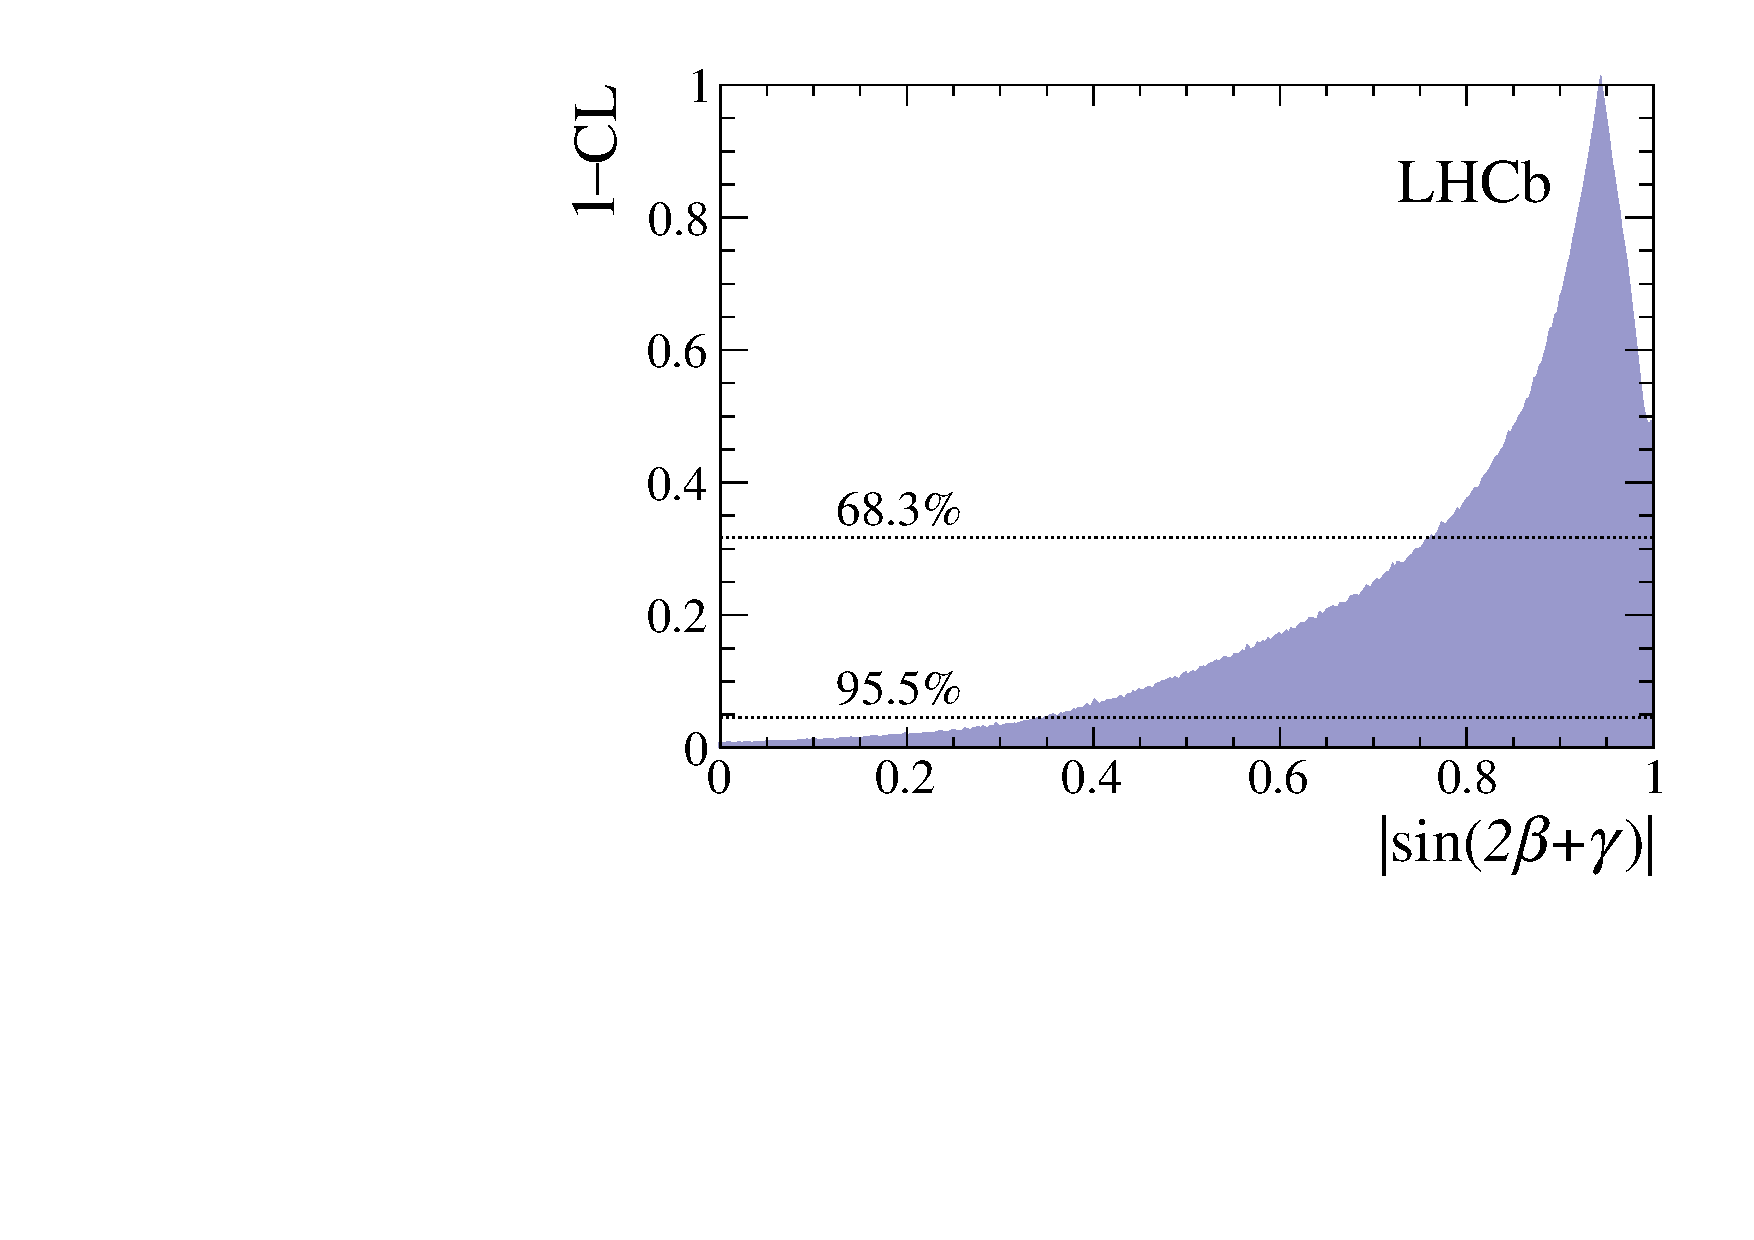
\includegraphics[width=0.6\textwidth]{12Result/figs/Sin2BetaPGamma.pdf}
    \caption{Distribution of $1-\text{CL}$ for $\left|\sin\!\left(2\beta+\gamma\right)\right|$.}
    \label{fig:sin2betaplusGamma}
\end{figure}
\begin{figure}[tbp]
    \centering
    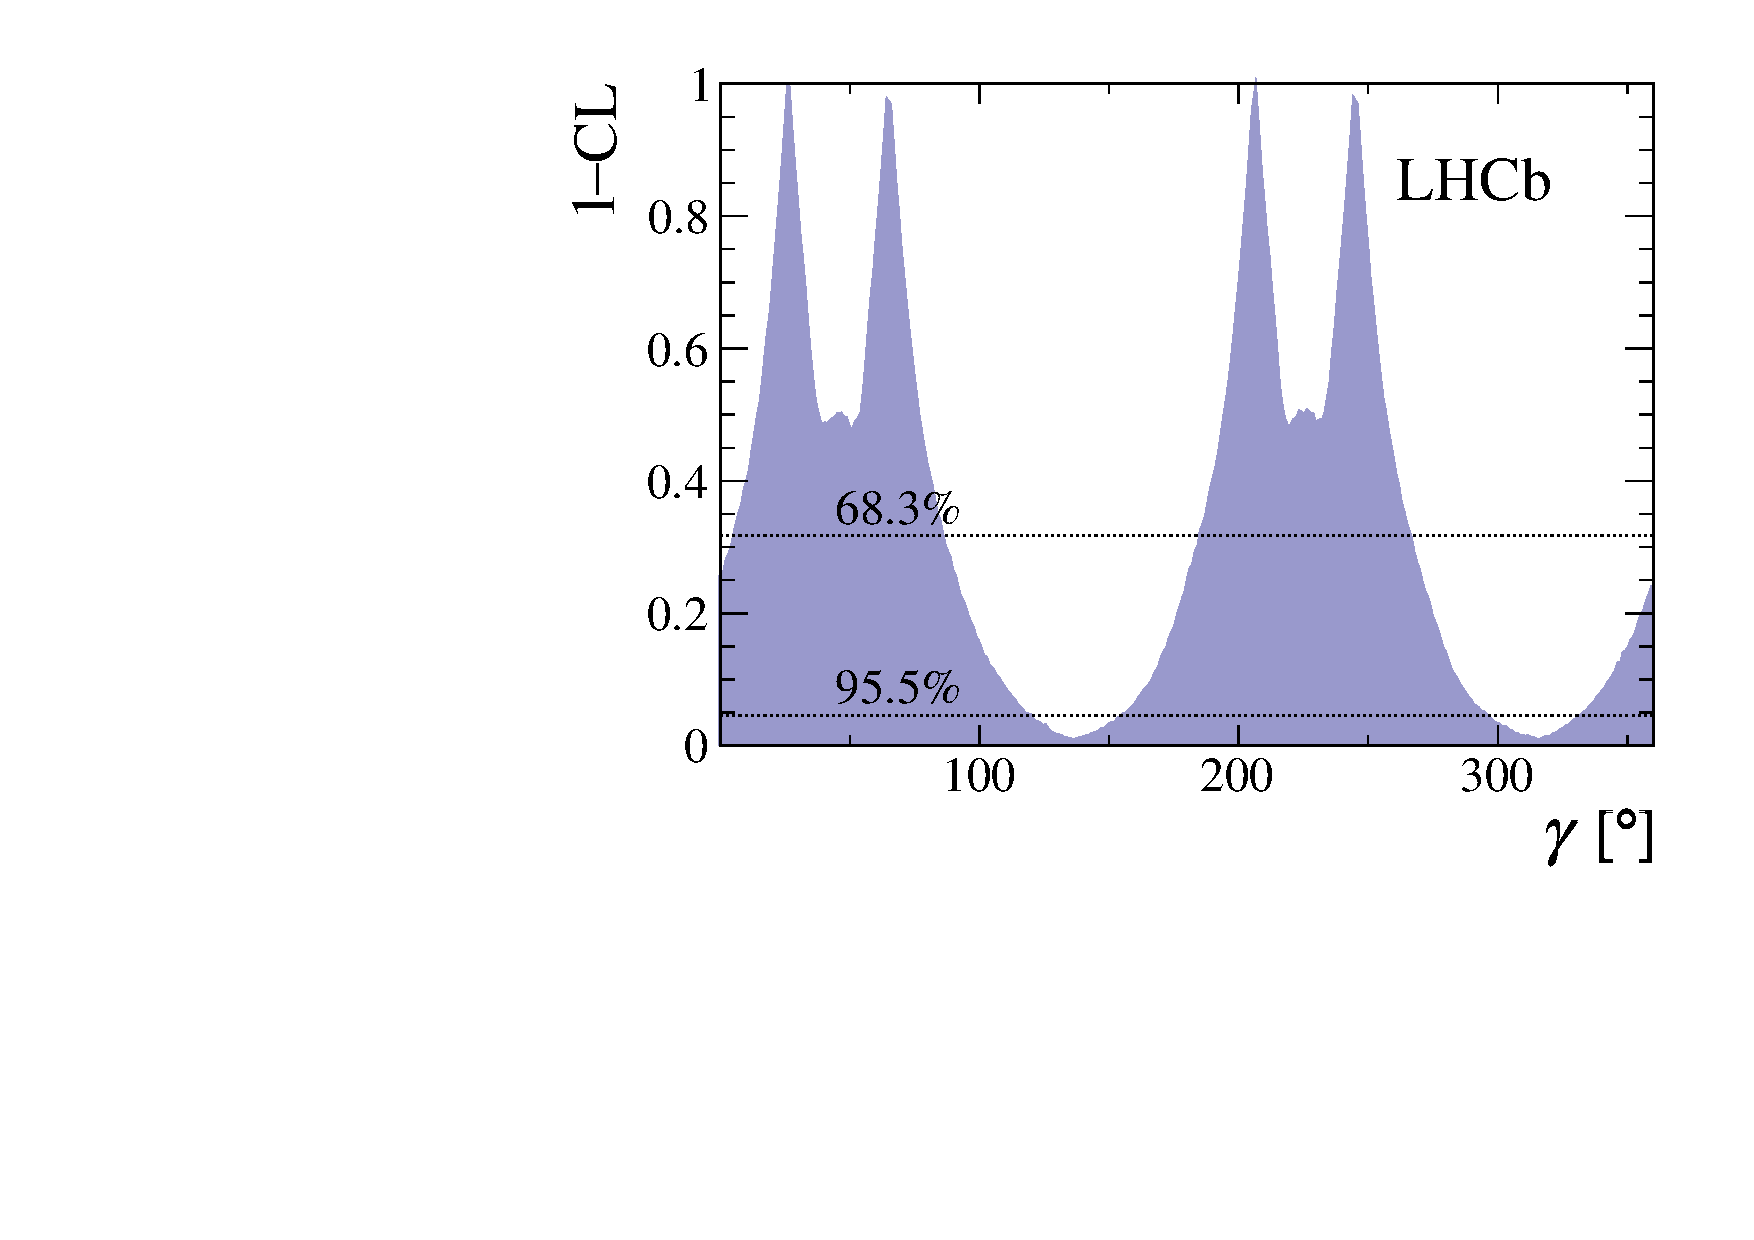
\includegraphics[width=0.48\textwidth]{12Result/figs/Gamma.pdf}
    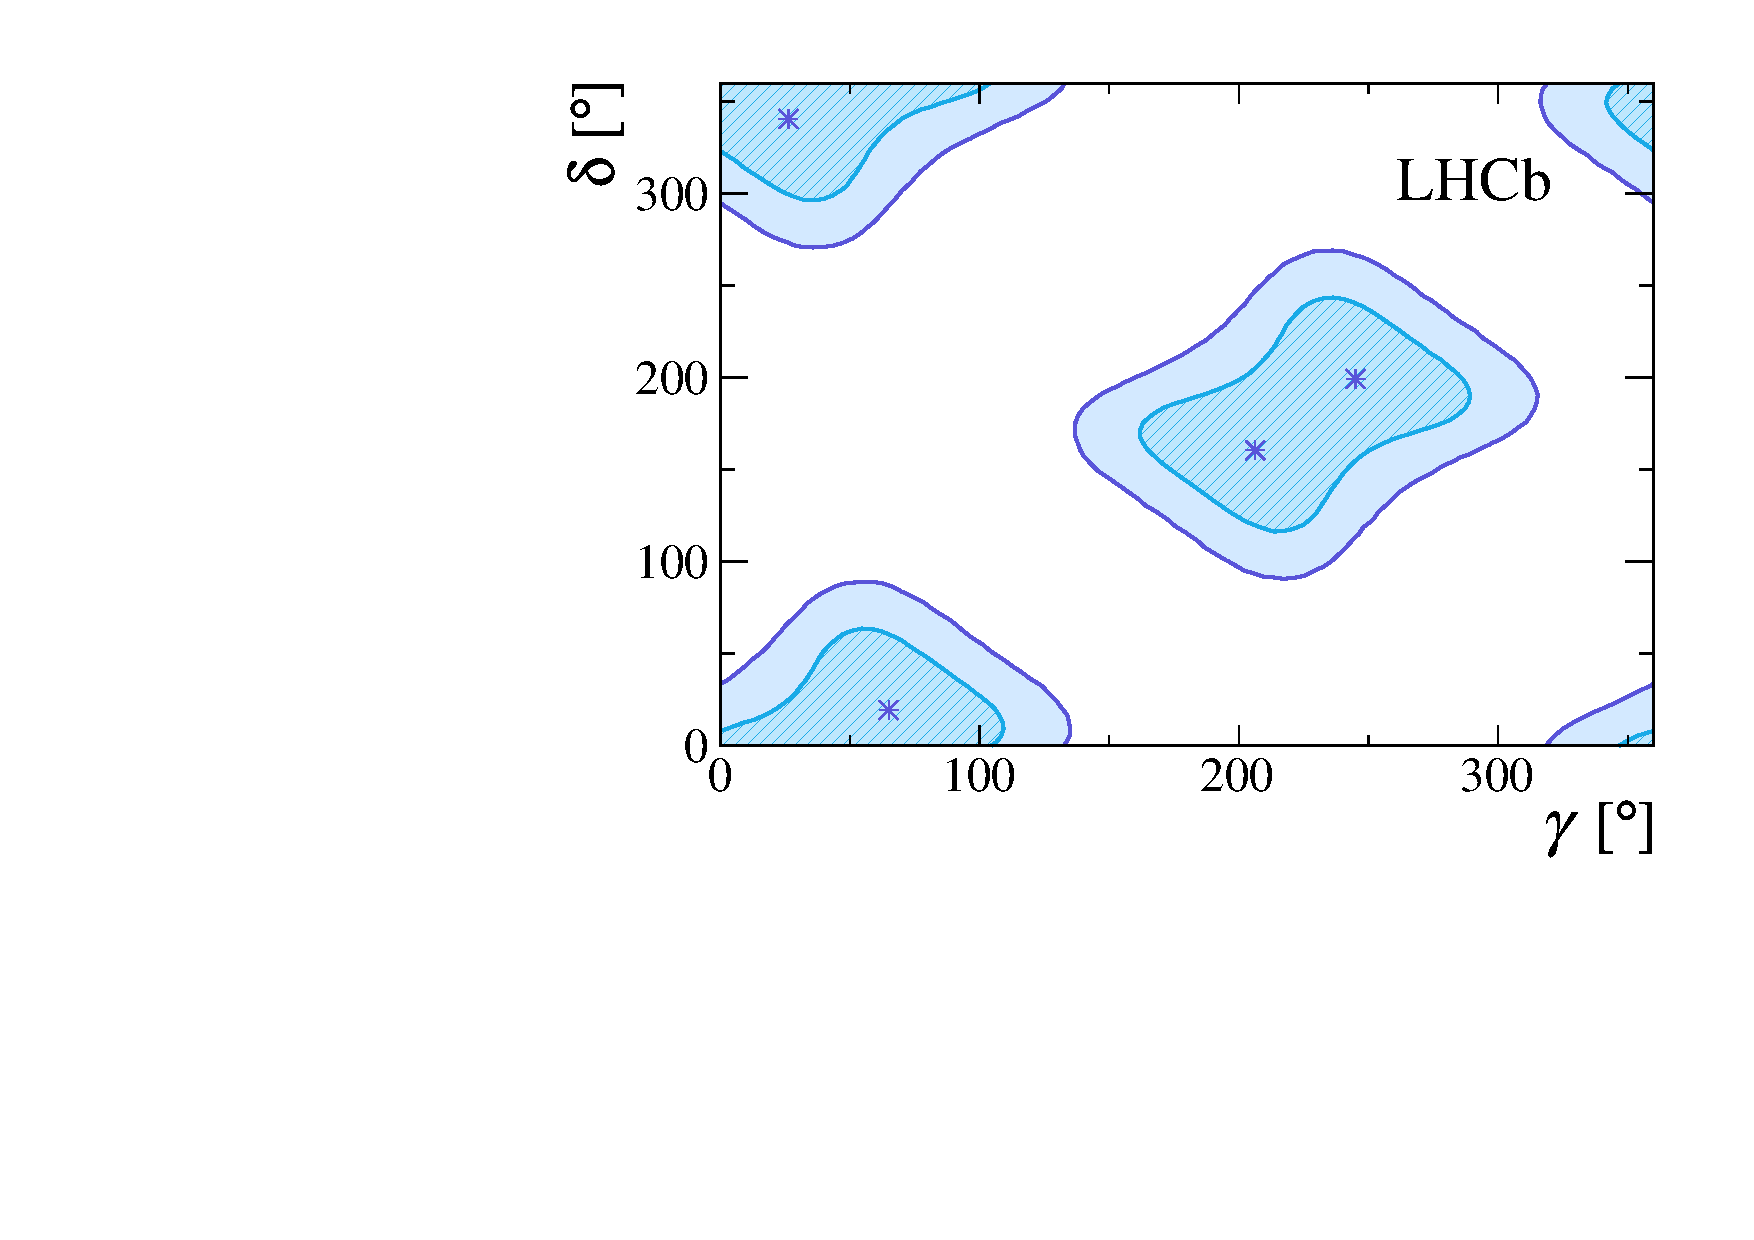
\includegraphics[width=0.48\textwidth]{12Result/figs/GammavsDelta.pdf}
    \caption{Distribution of $1-\text{CL}$ for $\gamma$ (left) and confidence regions for $\gamma$ vs. $\delta$ (right).
    The regions hold the \SI{39}{\percent} and \SI{87}{\percent} CL, the points denote the obtained maxima.}
    \label{fig:GammaAndGammavsdelta}
\end{figure}
The $1-\text{CL}$ interval for $\left|\sin\!\left(2\beta+\gamma\right)\right|$ is in agreement with, and more precise than, the previous measurements from the \belle and \babar collaborations~\cite{Ronga:2006hv,Aubert:2006tw}, also the distribution of the $1-\text{CL}$ shows the expected shape.
The result for $\gamma$ is compatible with all direct and indirect determinations presented in \cref{sec:comparisonGammaDeterms}.
However, the uncertainty is still quite large, so that on the one hand the precision of the measurement needs to be improved to make a conclusive statement about the agreement and on the other hand the contribution of this measurement to a combination of tree-level determinations of the angle $\gamma$ is very small~\cite{GammCombo}.
The obtained value for $\delta$ is compatible with the measured value in the time-dependent measurement of \CP violation using \BsToDsK decays~\cite{Aaij:2017lff}, which are related to \BdToDpi via the SU(3) symmetry~\cite{Fleischer:2003yb}.
The distributions of $1-\text{CL}$ for $\gamma$ and $\delta$ show the four-fold (two-fold) ambiguity for the range $[0, 360]\degrees$ ($[0, 180]\degrees$), which was discussed in \cref{sec:GammaInBd2Dpi}.
The uncertainties on $r$ and $\beta$ have a negligible impact on the confidence intervals.

As especially the assumption on SU(3) symmetry is highly unknown, the intervals are also determined for assumptions of \SI{0}{\percent}, \SI{20}{\percent} and \SI{100}{\percent} for the SU(3) breaking uncertainty of $r$.
These are representatively presented for $\gamma$ and $\left|\sin\!\left(2\beta+\gamma\right)\right|$ in \cref{fig:SU3Scan}, which shows that also assuming a larger uncertainty on the SU(3) symmetry yields reasonable confidence intervals.
\begin{figure}[tbp]
    \centering
    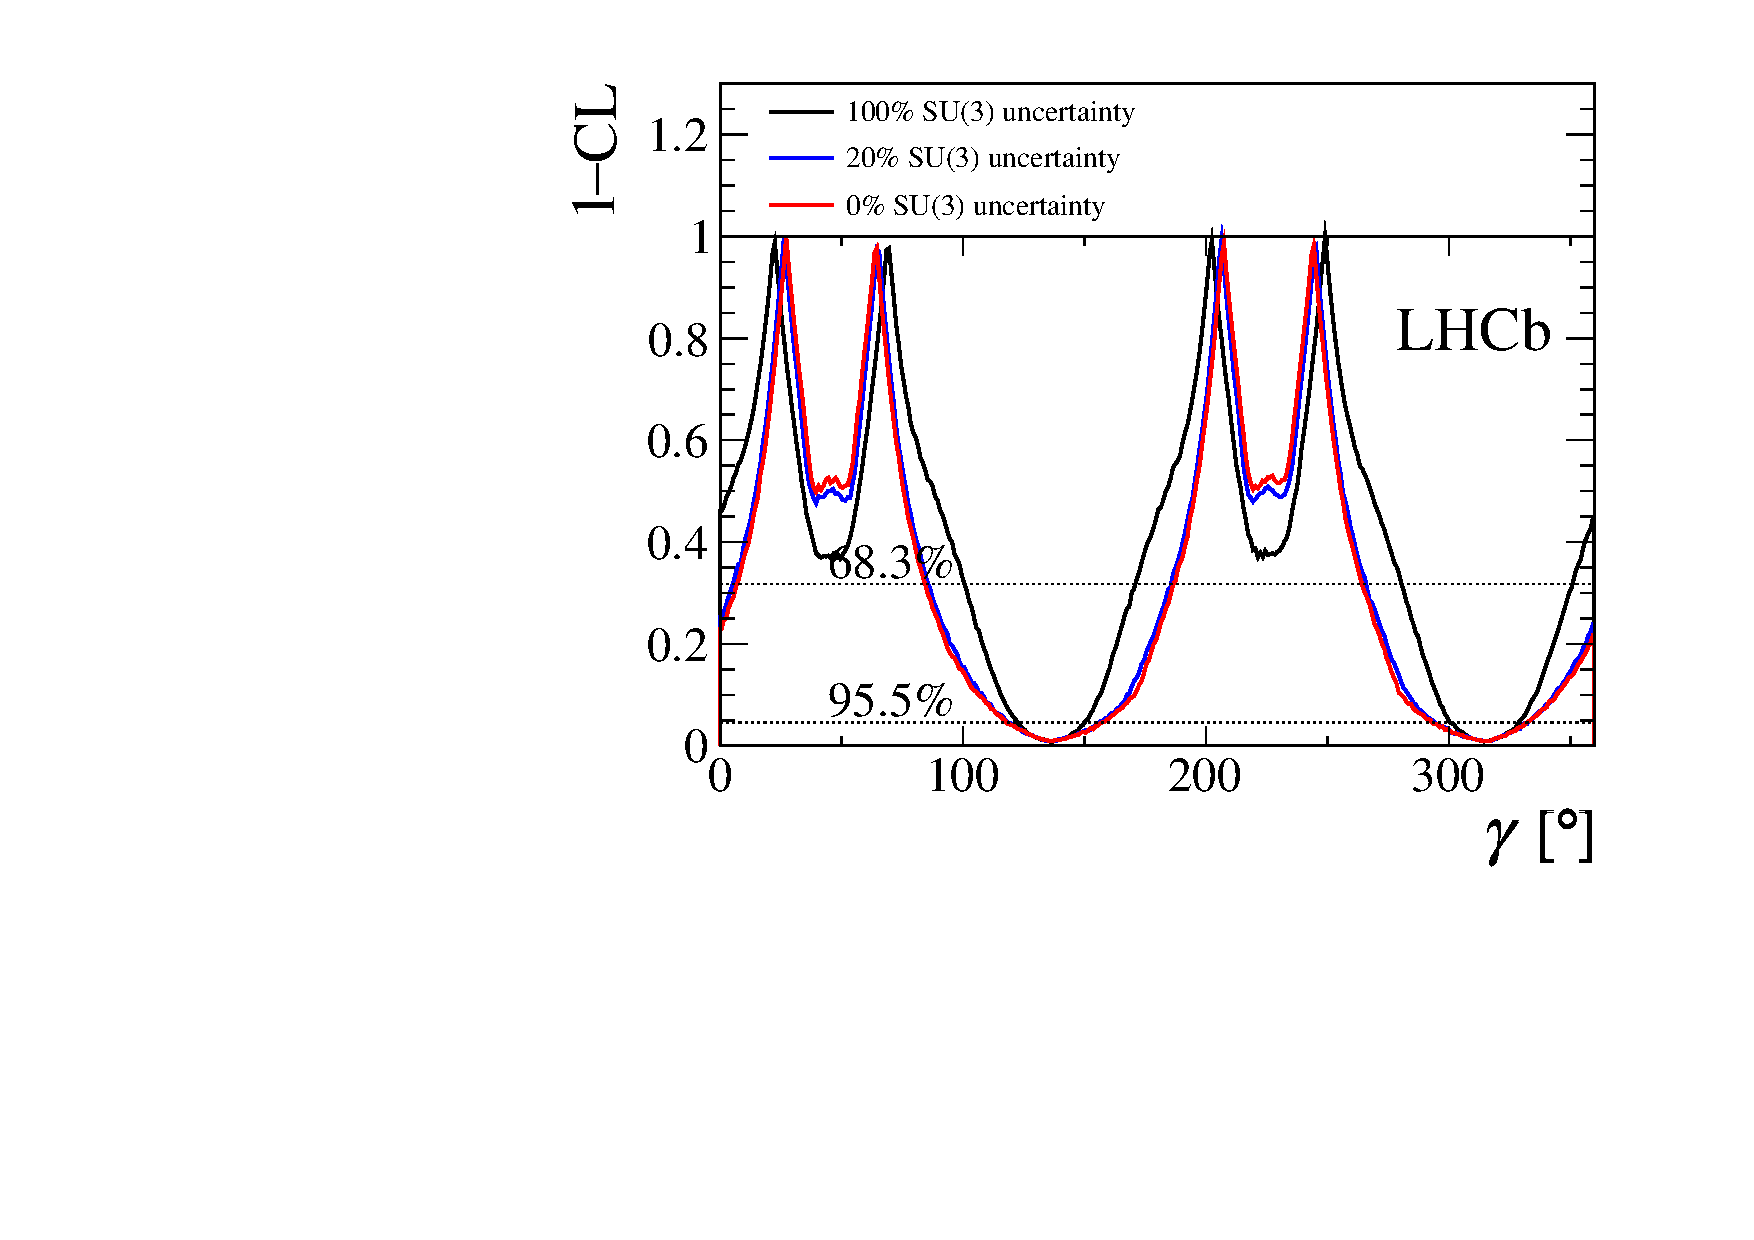
\includegraphics[width=0.48\textwidth]{12Result/figs/su3_scan_bd2dpi_g.pdf}
    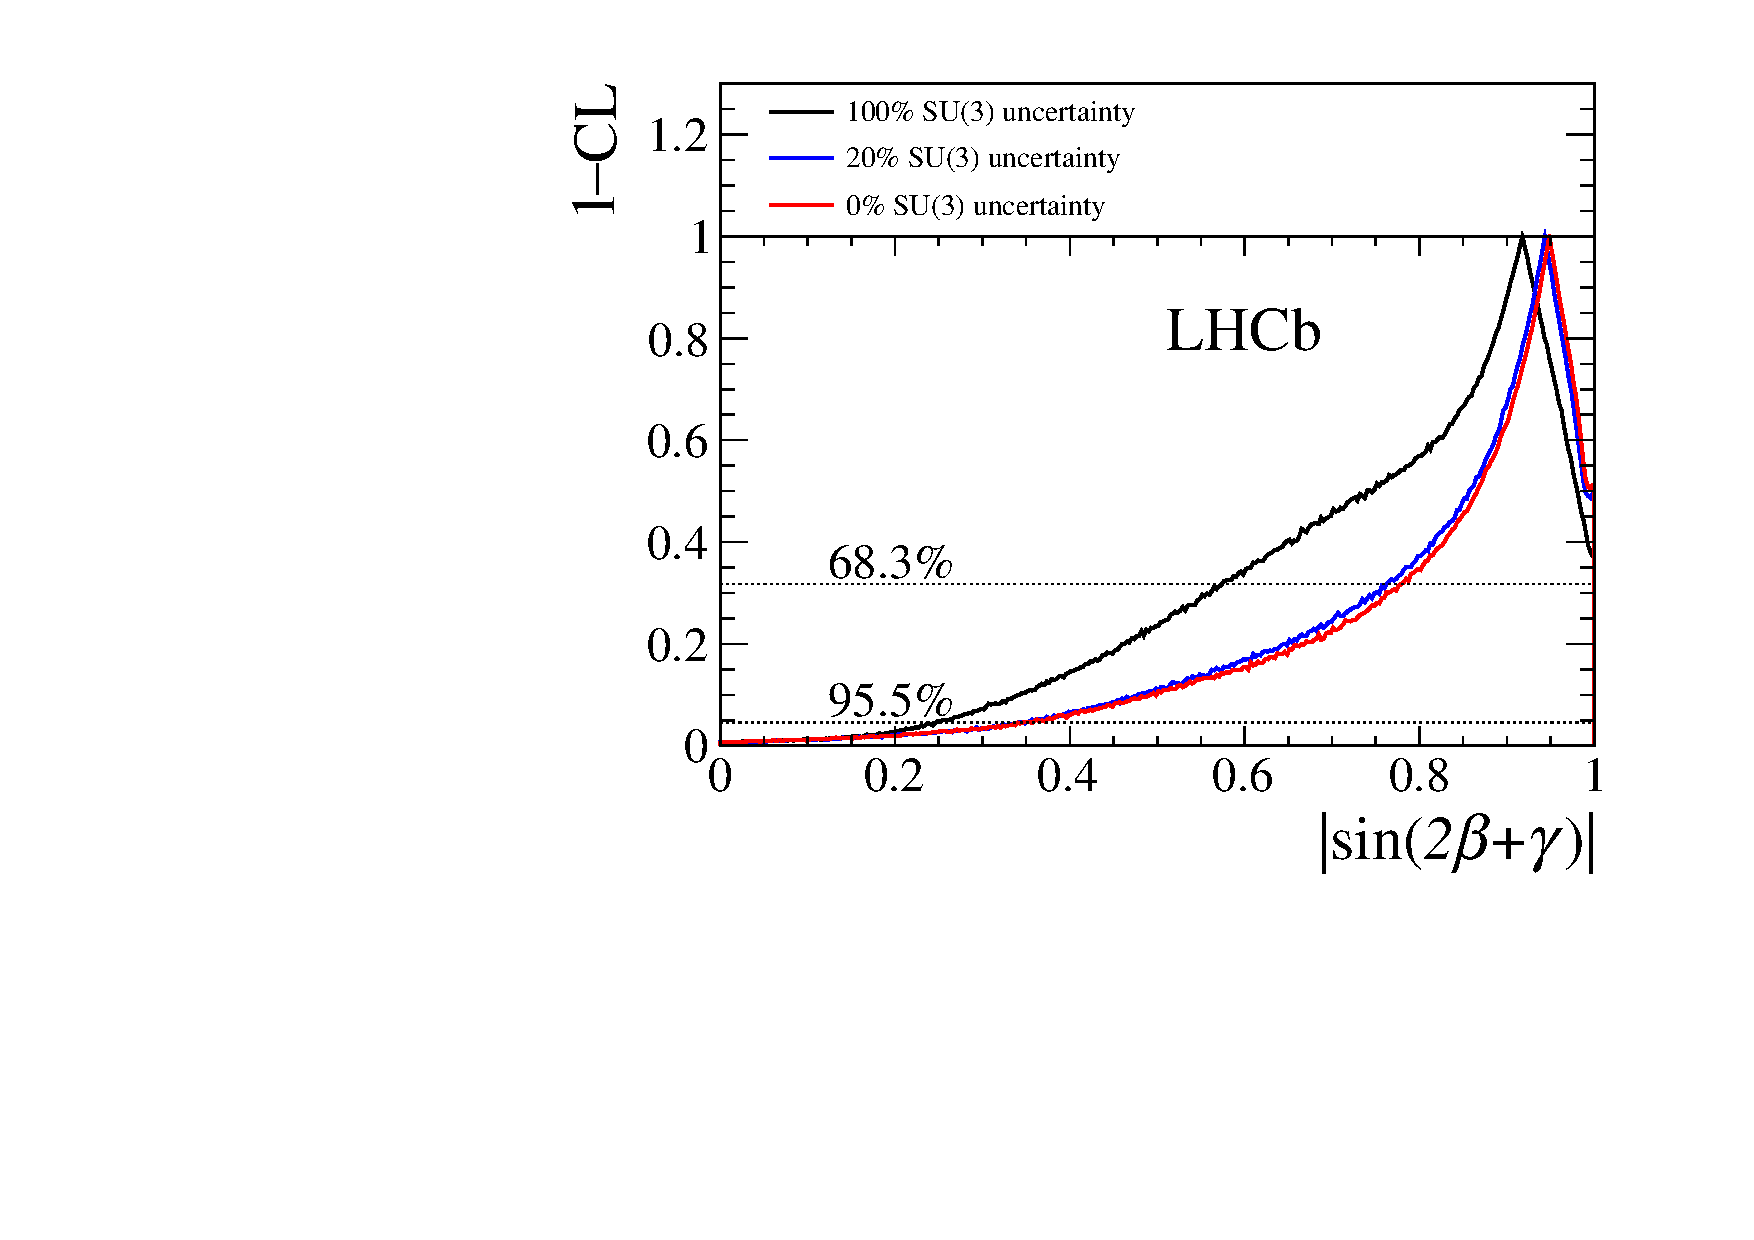
\includegraphics[width=0.48\textwidth]{12Result/figs/su3_scan_sin2b_plus_gamma.pdf}
    \caption{Distribution of $1-\text{CL}$ for $\gamma$ (left) and $\left|\sin\!\left(2\beta+\gamma\right)\right|$ (right) for assumptions of \SI{0}{\percent}, \SI{20}{\percent} and \SI{100}{\percent} for the SU(3) breaking uncertainty of $r$.}
    \label{fig:SU3Scan}
\end{figure}
